\PassOptionsToPackage{table}{xcolor}
\documentclass[9pt,xcolor=x11names,compress]{beamer}

%% General document %%%%%%%%%%%%%%%%%%%%%%%%%%%%%%%%%%
\usepackage{graphicx}
\usepackage{tikz}
\usepackage{array}
\usetikzlibrary{decorations.fractals,lindenmayersystems,shadings}
%%%%%%%%%%%%%%%%%%%%%%%%%%%%%%%%%%%%%%%%%%%%%%%%%%%%%%


%% Beamer Layout %%%%%%%%%%%%%%%%%%%%%%%%%%%%%%%%%%
\useoutertheme[subsection=false,shadow]{miniframes}
\useinnertheme{default}
\usefonttheme{serif}
\usepackage{palatino}

\setbeamerfont{title like}{shape=\scshape}
\setbeamerfont{frametitle}{shape=\scshape}

\setbeamercolor*{lower separation line head}{bg=DeepSkyBlue4} 
\setbeamercolor*{normal text}{fg=black,bg=white} 
\setbeamercolor*{alerted text}{fg=DeepSkyBlue4} 
\setbeamercolor*{example text}{fg=black} 
\setbeamercolor*{structure}{fg=black} 

\setbeamercolor*{palette tertiary}{fg=black,bg=black!10} 
\setbeamercolor*{palette quaternary}{fg=black,bg=black!10} 

\setbeamertemplate{blocks}[rounded][shadow=true]
\setbeamercolor{block title}{bg=DeepSkyBlue4}
\setbeamercolor{block title example}{bg=DeepSkyBlue4}
\setbeamercolor{block body}{bg=black!15!white}
\setbeamercolor{block body example}{bg=black!15!white}

\setbeamertemplate{navigation symbols}{}
%%%%%%%%%%%%%%%%%%%%%%%%%%%%%%%%%%%%%%%%%%%%%%%%%%
% Some useful definitions
\newcommand*\Laplace[1]{\mathcal{L}\{{#1}\}}
\newcommand*\BLaplace[1]{\mathcal{L}\Big\{{#1}\Big\}}
\newcommand*\iLaplace[1]{\mathcal{L}^{-1}\{{#1}\}}
\newcommand*\ibLaplace[1]{\mathcal{L}^{-1}\big\{{#1}\big\}}
\newcommand*\iBLaplace[1]{\mathcal{L}^{-1}\Big\{{#1}\Big\}}
%%%%%%%%%%%%%%%%%%%%%%%%%%%%%%%%%%%%%%%%%%%%%%%%%%

\author[Francisco Blanco-Silva]{Francisco Blanco-Silva}
\institute[USC]{University of South Carolina}
\date{ 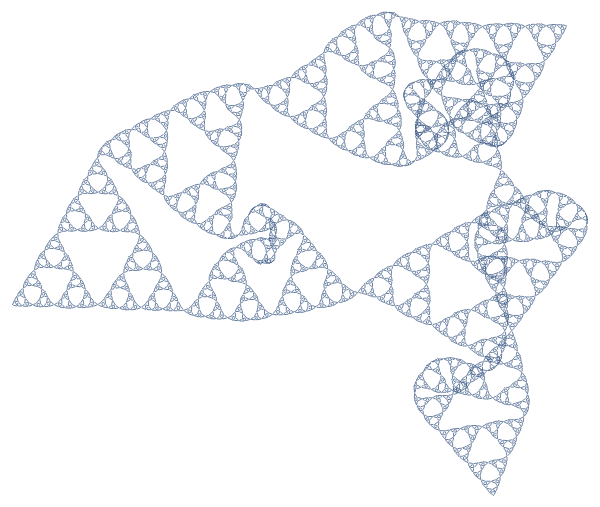
\includegraphics[width=0.45\linewidth]{lesson21ma242pic.png} }

\title{Lesson 21: Systems of Differential Equations: Introduction. Reduction to first-order systems.} 

\begin{document}

\frame{\titlepage}

\section{What do we know?}
\subsection{General Program}

\begin{frame}\frametitle{What do we know?}
\begin{columns}[T]
\begin{column}{0.45\linewidth}
\begin{itemize}
\item The concepts of \alert{differential equation} and \alert{initial value problem}
\item The concept of \alert{order} of a differential equation.
\item The concepts of \alert{general solution}, \alert{particular solution} and \alert{singular solution}.
\item \alert{Slope fields}
\item Approximations to solutions via \alert{Euler's Method} and \alert{Improved Euler's Method}
\end{itemize} 
\end{column}
\begin{column}{0.55\linewidth}
\begin{itemize}
\item First-Order Differential Equations
\begin{itemize}
\item Separable equations 
\item Homogeneous First-Order Equations 
\item Linear First-Order Equations 
\item Bernoulli Equations 
\item General Substitution Methods
\item Exact Equations 
\end{itemize}
\item Second-Order Differential Equations
\begin{itemize}
	\item Reducible Equations
	\item General Linear Equations (Intro)
	\item Linear Equations with Constant Coefficients
	\begin{itemize}
		\item Characteristic Equation
		\item Variation of Parameters
		\item Undetermined Coefficients
	\end{itemize}
\end{itemize}
\end{itemize}
\end{column}
\end{columns}
\end{frame}

\begin{frame}\frametitle{What do we know?}
\framesubtitle{Laplace Transforms}

\noindent\begin{tikzpicture}
\node[scale=0.7]{
\rowcolors{2}{white}{gray!25!white}
	\begin{tabular}{|m{2cm}|m{3.2cm}l||m{2cm}|m{3.2cm}l|}
	\rowcolor{DeepSkyBlue4}
		$f(x)$\raisebox{0.5cm} & $\mathcal{L}\{f\}=\int_0^\infty e^{-sx}f(x)\, dx$\raisebox{0.5cm} & &
		$f(x)$\raisebox{0.5cm} & $\mathcal{L}\{f\}=\int_0^\infty e^{-sx}f(x)\, dx$\raisebox{0.5cm} & \\[0.4cm]
		$1$ & $\dfrac{1}{s}$\raisebox{0.6cm} & $s>0$ &
		$cf(x)\pm g(x)$ & $cF(s) \pm G(s)$\raisebox{0.4cm} & $s>max(a,b)$ \\[0.4cm]
		$x^p$ & $\dfrac{\Gamma(p+1)}{s^{p+1}}$\raisebox{0.6cm} & $s>0$ &
		$x^n f(x)$ & $(-1)^n F^{(n)}$\raisebox{0.4cm} & $s>a$ \\[0.4cm]
		$x^n$ & $\dfrac{n!}{s^{n+1}}$\raisebox{0.6cm} & $s>0$ & $e^{\alpha x}f(x)$ & $F(s-\alpha)$\raisebox{0.4cm} & $s>a+\alpha$ \\[0.4cm]
		$e^{\alpha x}$ & $\dfrac{1}{s-\alpha}$\raisebox{0.6cm} & $s>\alpha$ & $\dfrac{f(x)}{x}$ & $\displaystyle{\int_s^\infty F(\sigma)\, d\sigma}$\raisebox{0.4cm} & $s>a$ \\[0.4cm]
		$\sin \beta x$ & $\dfrac{\beta}{s^2+\beta^2}$\raisebox{0.6cm} & $s>0$  &
		$f\star g$ & $F(s) G(s)$\raisebox{0.4cm} & $s>\max(a,b)$ \\[0.4cm]
		$\cos \beta x$ & $\dfrac{s}{s^2+\beta^2}$\raisebox{0.6cm} & $s>0$ & $f'(x)$ & $s F(s) -f(0)$\raisebox{0.4cm} & $s>a$ \\[0.4cm]
		\hline
		\end{tabular}};
	\end{tikzpicture}
\end{frame}

\section{Systems of Differential Equations}
\subsection{Introduction}

\begin{frame}\frametitle{Systems of Differential Equations}
    
\framesubtitle{Definition}
A system of differential equations is a collection of functions and functional equations of the form
\begin{equation*}
\underbrace{\begin{cases}
	y_1^{(n)} = F_1\big(x,y_1,y'_1,\dotsc,y_1^{(n-1)}, y_2,y'_2,\dotsc,y_2^{(n-1)},\alert{\dotsb},y_r,y'_r,\dotsc,y_r^{(n-1)}\big) \\
	y_2^{(n)} = F_2\big(x,y_1,y'_1,\dotsc,y_1^{(n-1)}, y_2,y'_2,\dotsc,y_2^{(n-1)},\alert{\dotsb},y_r,y'_r,\dotsc,y_r^{(n-1)}\big) \\
	\dotsc\\
	y_r^{(n)} = F_r\big(x,y_1,y'_1,\dotsc,y_1^{(n-1)}, y_2,y'_2,\dotsc,y_2^{(n-1)},\alert{\dotsb},y_r,y'_r,\dotsc,y_r^{(n-1)}\big)
\end{cases}}_{\text{order }n, r\text{ functions}}
\end{equation*}
\pause Some examples
\begin{equation*}
	\underbrace{\begin{cases}
		y'_1=x+y_1-y_2 \\
		y'_2=2y_1-3y_2
	\end{cases}}_{\text{first order, two functions}}\qquad
	\uncover<3->{\underbrace{
	\begin{cases}
		y''_1=y_2+y'_3 \\
		y''_2=y_3-y'_1 \\
		y''_3=y_1+y'_2
	\end{cases}}_{\text{second order, three functions}}}
\end{equation*}
\end{frame}

\subsection{Transformation to first-order systems}

\begin{frame}\frametitle{Systems of Differential Equations}
\framesubtitle{Transformation to first-order systems}
Any differential equation of order $n$ can be transformed into a system of $n$ differential equations of first order:
\begin{equation*}
	y^{(n)}=F(x,y,y',y'',\dotsc,y^{(n-1)})
\end{equation*}
\pause We start by assigning $y_1=y$ and, to each $k$-th derivative of $y$, the function $y_{k+1}$:
\begin{equation*}
	y_1=y,\quad y_2=y',\quad y_3=y'',\quad \dotsc\quad y_n=y^{(n-1)}
\end{equation*}
\pause Note that now, $y'_1=y'=y_2$, $y'_2=y_3$ and, in general, $y'_k=y_{k+1}$.  We have the system we required:
\begin{equation*}
	\begin{cases}
		y'_1=y_2\\
		y'_2=y_3\\
		\dotsb \\
		y'_{n-1}=y'_n \\
		y'_n=y^{(n)}=F(x,y,y',y'',\dotsc,y^{(n-1)})=F(x,y_1,y_2,\dotsc,y_n)
	\end{cases}
\end{equation*}
\end{frame}

\begin{frame}\frametitle{Systems of Differential Equations}
\framesubtitle{Examples}
\begin{block}
	{Transform the differential equation in a first-order system of differential Equations}
	\begin{equation*}		
		y'''+3y''+2y'-5y=\sin 2x	
	\end{equation*}		
\end{block}
\pause We start with the assignment of functions first.  We stop at three (the order of the differential equation)
\begin{equation*}
	y_1=y,\qquad y_2=y',\qquad y_3=y''
\end{equation*}
\pause We take derivatives now.  \alert{\uncover<6->{Note that $y'_3=y'''=\sin 2x+5y-2y'-3y''$}}
\pause \begin{equation*}
	\begin{cases}
		\uncover<4->{y'_1=y_2 \\}
		\uncover<5->{y'_2=y_3 \\}
		\uncover<6->{y'_3=\sin 2x + 5 y_1 - 2 y_2 -3 y_3}
	\end{cases}
\end{equation*}
\end{frame}

\begin{frame}\frametitle{Systems of Differential Equations}
    
\framesubtitle{Transformation to First-Order Systems}
Using the same technique, it is also possible to transform any system of differential equations into another of order one.
\pause \begin{block}
	{Transform the following system to First-order}
	\begin{equation*}
		\begin{cases}
				y''_1=-3y_1+y_2\\
				y''_2=2y_1-2y_2+40\sin 3x
			\end{cases}	
	\end{equation*}
\end{block}
\pause We proceed to label $Y_1=y_1$, $Y_2=y'_1$, $Y_3=y_2$ and $Y_4=y'_2$.  We have then
\begin{equation*}
	\begin{cases}
		\uncover<4->{Y'_1=Y_2\\}
		\uncover<5->{Y'_2=-3Y_1+Y_3\\}
		\uncover<6->{Y'_3=Y_4\\}
		\uncover<7->{Y'_4=2Y_1-2Y_3+40\sin 3x}
	\end{cases}
\end{equation*}
\end{frame}

\begin{frame}\frametitle{Systems of Differential Equations}
\framesubtitle{Examples}
It is often possible to solve a first-order system of differential equations by transforming it to a single differential equation.
\pause \begin{block}
{Transform the following system into a differential equation, and solve it}
\begin{equation*}
	\begin{cases}
		y'_1=-2y_2 \\
		y'_2=\frac{1}{2}y_1
	\end{cases}
\end{equation*}
\end{block}
\pause Note that 
\begin{equation*}
	y''_1=-2y'_2\uncover<4->{=-2\big(\tfrac{1}{2}y_1\big)=-y_1}
\end{equation*}
\pause\pause We have then the second order homogeneous linear equation with constant coefficients $y''_1+y_1=0$, with general solution 
\begin{equation*}
y_1=A\cos x+B\sin x
\end{equation*}
\pause It must be then 
\begin{equation*}
y_2=-\tfrac{1}{2}y'_1\uncover<7->{=\tfrac{A}{2}\sin x - \tfrac{B}{2}\cos x}
\end{equation*}
\end{frame}

\begin{frame}\frametitle{Systems of Differential Equations}
    
\framesubtitle{Examples}
\begin{block}
	{Transform the system into a differential equation, and solve it}
	\begin{equation*}
		\begin{cases}
			y'_1=y_2\\
			y'_2=2y_1+y_2
		\end{cases}
	\end{equation*}
\end{block}
\pause As before, we start by taking derivatives of the easier equation:
\begin{equation*}
	\alert{y''_1}=y'_2=2y_1+y_2\uncover<3->{=\alert{2y_1+y'_1}}
\end{equation*}
\uncover<4->{We have the second-order homogeneous linear equation with constant coefficients}
\begin{equation*}
	\uncover<4->{y''_1-y'_1-2y_1=0}
\end{equation*}
\uncover<5->{The general solution is readily found from the roots of the characteristic equation:}
\begin{equation*}
	\uncover<5->{r^2-r-2=0,\qquad r=\frac{1\pm \sqrt{1-4\cdot(-2)}}{2}=\frac{1\pm 3}{2}=\{ 2, -1\}}
\end{equation*}
\uncover<6->{We have}
\begin{align*}
	\uncover<6->{y_1&=A e^{-x} + Be^{2x}}\\
	\uncover<7->{y_2&=y'_1=-Ae^{-x} + 2Be^{2x}}
\end{align*}
\end{frame}
\end{document}